\documentclass{article}

\usepackage{booktabs}
\usepackage{multirow}
\usepackage{amsmath}
\usepackage{hyperref}
\usepackage{overpic}
\usepackage{amssymb}
\usepackage{lipsum}

\usepackage[accepted]{dlai2021}

%%% STUDENTS: FILL IN WITH YOUR OWN INFORMATION
\dlaititlerunning{Ornithology expert system}

\begin{document}

\twocolumn[
%%% STUDENTS: FILL IN WITH YOUR OWN INFORMATION
\dlaititle{BirdCLEF2021: An ornithology expert system}

\begin{center}\today\end{center}

\begin{dlaiauthorlist}
%%% STUDENTS: FILL IN WITH YOUR OWN INFORMATION
\dlaiauthor{Edoardo De Matteis}{}
\end{dlaiauthorlist}

%%% STUDENTS: FILL IN WITH YOUR OWN INFORMATION
\dlaicorrespondingauthor{Edoardo De Matteis}{dematteis.1746561@studenti.uniroma1.it}

\vskip 0.3in
]

\printAffiliationsAndNotice{}

\begin{abstract}
In this report I approached the BirdCLEF2021 bird classification task and came up with a model that uses only soundscape recording, thus making most of the data privileged, and getting good results.
The code is available on GitHub at \href{https://github.com/edodema/Birdcalls}{https://github.com/edodema/Birdcalls}
\end{abstract}

\section{Introduction}
Birds are sensitive to changes in the ecosystem due to them being high up in the food chain, so monitoring them can give us informations about pollution and the environment.
While small birds are often difficult to sight they tend to sing a lot, and these calls are generally characteristic of each species, that's why a smart way to identify them is through their call.
Our goal is to guess a bird's species by its call in a noisy recording, the task is set up as an image classification among $n+1$ classes i.e. $n$ species plus no bird being detected. 

\paragraph*{Dataset.}
The BirdCLEF2021 dataset contains recordings of both birds in a controlled environment and noisy soundscapes,  the  latters  being  split  in  5  seconds  windows  and labeled with primary and secondary labels.
For our purposes I only considered primary labels, that should not be a problem since we are just being conservative, secondary ones are just some of the privileged data that we will ignore, in fact we will not use birds recordings at all and still get good results.

\section{Related work}
Many previous works have exploited spectrograms to reduce audio recognition to an image task ~\cite{hamdyaudio} ~\cite{michelashvili2020denoising} ~\cite{xie2021audio}, among them ~\cite{xie2021audio} uses a recurrent layer to extrapolate time sensitive knowlgedge.
In the same way we canuse attention and one of the basic blocks that will form our model has been inspired by ~\cite{zhang2020resnest}, in which a variation of \textit{ResNet} ~\cite{he2016deep} with split-attention is developed.
Also from \textit{ResNet} itself I took some numerical techniques to stabilize results.

\section{Method}
What happens when ornithologists recognize a birdcall, do they first detect a sound and then focus to classify it or does their brain automatically recognize the bird species?
It makes sense to believe it is possible to be so proficient to unconsciously recognize birds, as already happens with familiar sounds ~\cite{kirmse2009familiarity}. 
Let's call the first approach \textit{split} and the second one \textit{joint}, I tried both of them but only the latter model is covered here due to computational issues with the first one (for those interested, results are still shown on the GitHub repository).

\paragraph*{Preprocessing.}
The dataset recordings, regardless of bird calls or soudscapes, are highly unbalanced (figure \ref{fig:soundscapes_classification_freq}), that's why the dataset is augmented by random oversampling.
Then it is split in train, validation and test sets by a 80-10-10 ratio and each 5 seconds window in audio tracks is encoded as a spectrogram in mel scale.
Transforming spectrograms (e.g. random crops) could have led to losing positive data (i.e. a bird singing) and keeping silence, or vice versa, leading to wrong labeling; even if that did not happen it would have not been strange to lose relevant data, due to the task being modeled as seq2seq.   
Anyway due to computing limitation it was not possible to use all the data so a smaller split of randomly selected data was used during training.

\begin{figure}
    \centering
    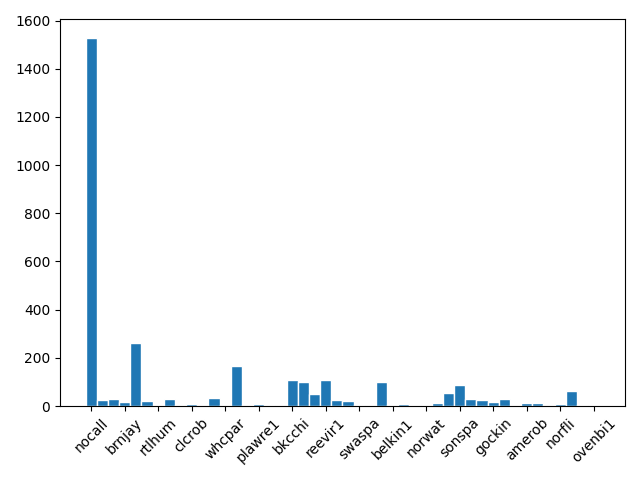
\includegraphics[scale=.35]{images/soundscapes_distribution_birds.png}
    \caption{Primary label distribution in soundscape recordings.}
    \label{fig:soundscapes_classification_freq}
\end{figure}

\paragraph*{CNNAtt.}
This custom defined layer expoits multi-head attention layers to build a seq2seq model with the intent to grasp time-series knowledge.
First the spectrogram passes through three different convolution pipelines, each one used respectively as a query, key and value for the attention.
The RNNs in the attention layers work on tensor rows independently, this means that we would learn looking at frequencies with no connection whatsoever between them, thus a second attention layer works on transposed spectrograms' feature images.
The two representations are then concatenated to get a 2 channel image.
As a note, when we refer to a CNNAtt$k$ block it means that convolutions have all the same kernel size $k$.

\begin{figure}
    \centering
    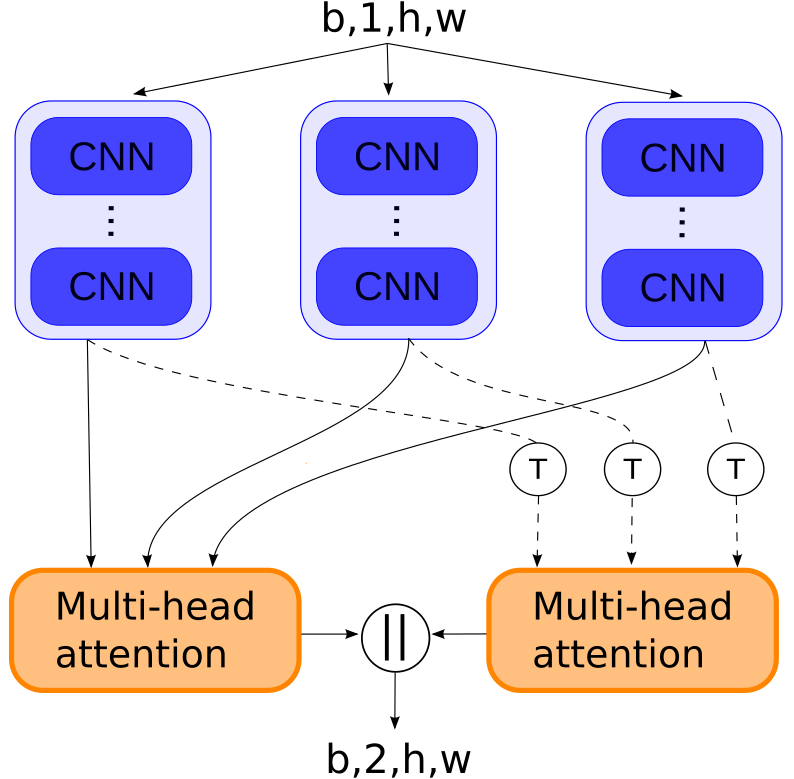
\includegraphics[scale=.3]{images/cnn_att.png}
    \caption{A CNNAtt block.}
    \label{fig:cnnatt}
\end{figure}

\paragraph*{CNNRes.}
Residual networks are effective at reducing error when dealing with deep networks, and I tried one pretrained \textit{ResNet18} model as a feature extraction backbone.
Also this simpler residual network has been defined, it employs six convolutions of the same kernel size among with two residual paths between them (figure \ref{fig:cnnres}).
It takes inspiration by a \textit{ResNeSt} block ~\cite{zhang2020resnest}, but the number of cardinals is fixed to 3 to use them as keys, queries and values in the multi-head attention layer. 
Is possible to stack $n$ layers one on top of the other, in such cases we will write CNNRes$n$, as a rule the number of kernels stays the same when the feature map has the same size as the input image, and it is doubled when feature map has half the size of the image ~\cite{he2016deep}.
There are no residuals between different CNNRes block therefore there is no need in dealing with tensor with different shape. 

\begin{figure}
    \centering
    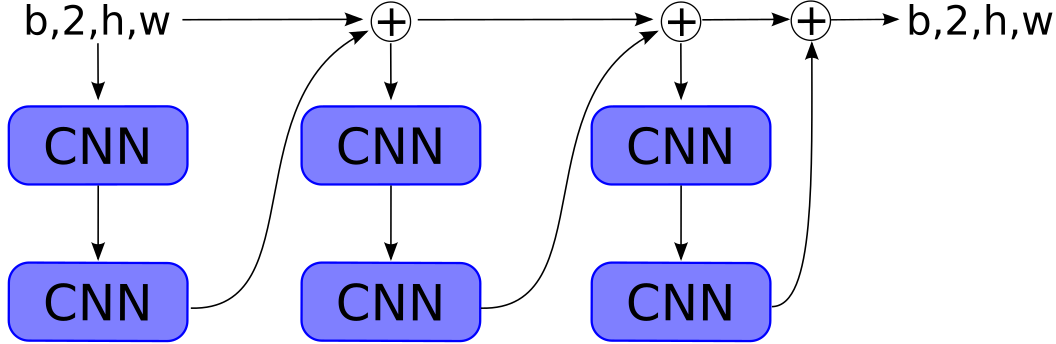
\includegraphics[scale=.25]{images/cnn_res.png}
    \caption{A CNNRes block.}
    \label{fig:cnnres}
\end{figure}

The afore mentioned layers build up the feature extraction backbone, between CNNAtt and CNNRes we have another convolution to deal with the number of filters.
After that we have $m$ bilinear GRU layers as a seq2seq model to extract other sequential knowledge, and last a linear layer to output logits.

In our experiments we use a cross entropy loss, and use both models build  from scratch i.e. CNNRes2 (with kernel sizes $3$ and $5$) and CNNAtt5CNNRes2 that adds a CNNAtt block to it, according to the afore-mentioned rules.
But we also fine-tune pretrained models \textit{ResNet18} and \textit{ResNet50}, with a convolution and a linear layer to match \textit{ResNet}s input and output shapes.

\section{Results}
Training has been done using an \textit{Adam} optimizer with $8$ samples per batch, primarly due to memory limitations but it turned out good sinc we get some nice spikes.
Results are reported at table \ref{tab:joint-results}, since datasets have been balanced and all classes are equally important it makes sense to use accuracy.

\begin{table}[h!]
    \caption{Performances are for the validation set with a fixed seed of 42, the test accuracy is reported for CNNRes2 only.}
    \label{tab:joint-results}
    \begin{center}
        \begin{small}
            \begin{tabular}{p{0.35\linewidth} | ccc}
                \toprule
                & \multirow{2}{0.13\linewidth}{LR} 
                & \multirow{2}{0.13\linewidth}{Loss $\downarrow$} 
                & \multirow{2}{0.13\linewidth}{Acc. $\uparrow$} \\
                Model \\
                \midrule
                ResNet18 & 1e-4 & .21 & 92.2\% \\
                ResNet50 & 1e-4 & .52 & 82.3\% \\
                CNNRes2 & 1e-4 & \textbf{.02} & \textbf{99.1\%} \\
                CNNAtt5 + CNNRes2 & 1e-4 & .04 & 98.7\% \\
                \midrule
                \midrule
                Test & - & - & 99.4\% \\
                \bottomrule
            \end{tabular}
        \end{small}
    \end{center}
    \vspace{-0.5cm}
\end{table}

\begin{figure}
    \centering
    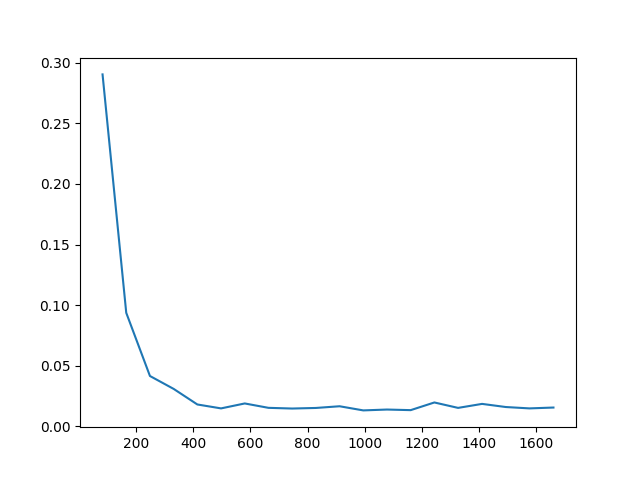
\includegraphics[scale=.5]{images/val_loss.png}
    \caption{Validation loss for CNNRes2GRU1FC1.}
    \label{fig:val-loss}
\end{figure}

Occam's razor holds and it seems that a simpler approach is the way to go, pretrained models are not very good but it can happen with transfer learning. 

\paragraph*{Future works.}
It would be nice to have enough resources to train on the whole dataset, this way we could also effectively try the split method.
Also adding a threshold as an hyperparameter we could consider secondary labels too.

\bibliography{references.bib}
\bibliographystyle{dlai2021}

\end{document}